\documentclass{bioinfo}
\copyrightyear{2014}
\pubyear{2014}

\usepackage{hyperref}

\begin{document}
\firstpage{1}

%\title[short Title]{Structure prediction of globular proteins using predicted residue contacts.}
%\title[short Title]{PconsFold: ab-initio protein folding using Rosetta and predicted residue contacts.}
\title[PconsFold]{PconsFold: Protein folding using predicted residue contacts}
%\title[short Title]{Advancement in residue contact prediction improves quality of predicted structural models.}
%\author[Sample \textit{et~al}]{Mirco Michel\,$^{1,2}$, Marcin J. Skwark\,$^{3}$ and Arne Elofsson\,$^{1,2}$\footnote{to whom correspondence should be addressed}}
\author[M.Michel \textit{et~al}]{Mirco Michel\,$^{1,2}$, Sikander Hayat, Marcin Skwark, Debora Marks, and Arne Elofsson\,$^{1,2}$\footnote{to whom correspondence should be addressed}}
\address{$^{1}$Department of Biochemistry and Biophysics, Stockholm University, 10691 Stockholm, Sweden\\
$^{2}$Science for Life Laboratory, Box 1031, 17121 Solna, Sweden\\
AFFILIATIONS}
%$^{3}$Department of Information and Computer Science, Helsinki University of Technology TKK, Box 5400, FI-02015 TKK, Finland}

\history{Received on XXXXX; revised on XXXXX; accepted on XXXXX}

\editor{Associate Editor: XXXXXXX}

\maketitle

\begin{abstract}

\section{Motivation:}

\section{Results:}
Here we show that improved quality of evolutionary constraints increases quality and native-likeliness of predicted models. We also show that 
\section{Availability:}
We provide a fully automated pipeline, PconsFold, for predicting protein structures based on evolutionary information. PconsFold is based on PconsC and Rosetta and freely available at \url{https://www.github.com/ElofssonLab/pcons-fold}.
\section{Contact:} \href{arne@bioinfo.se}{arne@bioinfo.se}
\end{abstract}

\section{Introduction}
The protein folding problem is one of the longest standing problems in structural biology. Although the problem itself remains unsolved, there has been continuous effort and progress resulting in increased accuracy of predicted models \cite[]{kryshtafovych_CASP10_2013}. \\\indent
The idea of using predicted residue-residue contacts for protein structure prediction is not new \cite[]{CITATION NEEDED}. However, until recently \cite[]{marks_protein_2011} predicted contacts lacked the accuracy to facilitate structure prediction methods significantly. This only became possible due to a new approach to separate direct from indirect contact information \cite[]{burger_disentangling_2010}. Since then there has been continuous effort to improve the quality of predicted contacts \cite[]{morcos_direct-coupling_2011, jones_PSICOV:_2012, ekeberg_improved_2013, skwark_PconsC:_2013} and to apply such contacts in structure prediction of membrane proteins \cite[]{hopf_three-dimensional_2012, nugent_accurate_2012}. Although the utility of current contact prediction methods is limited \cite[]{kamisetty_assessing_2013}, we want to highlight the importance of such information in cases where it is applicable. \\\indent
\begin{figure}[!tpb]%figure1
\centerline{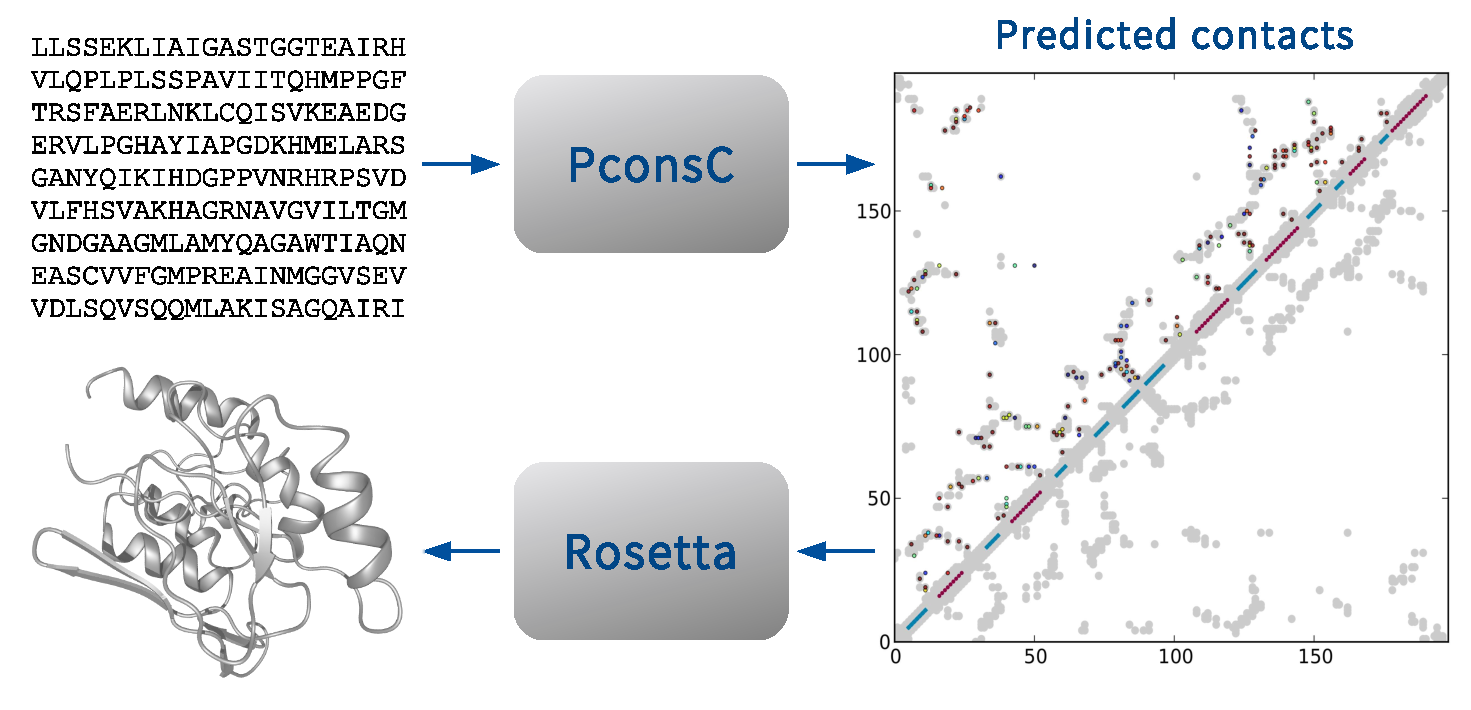
\includegraphics[scale=0.35]{figures/pipeline.eps}}
\caption{PconsFold pipeline. Based on a given protein sequence, amino-acid contacts are predicted with PconsC. These contacts then facilitate protein folding with Rosetta. In the end PconsFold outputs a structural model for the given sequence.}\label{fig:pipeline}
\end{figure}
Here we show that improved quality of predicted contacts increases quality and native-likeliness of predicted structures. We developed PconsFold, a pipeline for ab-initio protein structure prediction of globular single-domain proteins (Figure \ref{fig:pipeline}). PconsFold is based on predicted amino-acid contacts from PconsC. These contacts are utilized within Rosetta to fold a given protein sequence from scratch. We benchmark our method on two datasets and compare it to EVfold \cite[]{marks_protein_2011}, a previous method for contact based protein structure prediction. The source code for PconsFold is available on GitHub (\url{https://www.github.com/ElofssonLab/pcons-fold}) under the MIT license.

\begin{methods}
\section{Methods}

\subsection{Datasets}
During the development of PconsFold we used the proteins from \citeauthor{jones_PSICOV:_2012} \citeyear{jones_PSICOV:_2012} (PSICOV dataset). It consists of 150 single domain proteins with sequence lengths between 75 and 275 amino acids. A list of all Protein Data Bank (PDB) \cite[]{berman_protein_2000} and corresponding Uniprot \cite[]{magrane_uniprot_2011} IDs is given in (Supplementary Table T1). \\\indent
For each protein we chose to use its PDB seqres sequence as input and not its atom sequence. This avoids internal gaps due to missing residues in the crystal structure. We chose not to use Uniprot sequences directly due to mutations and other sequential differences to the PDB sequences. This allows direct comparisons between predicted models and native PDB structures. Taking account for structural differences due to diverging sequences is thus not necessary. \\\indent
For the final comparison between PconsFold and EVfold we used the set of 15 proteins as in \citeauthor{marks_protein_2011} \citeyear{marks_protein_2011} . PDB and Uniprot IDs are given in Supplementary Table T2. Here we used the exact same sequences and native structures as given in the publication.

\subsection{Contact prediction}
In case of PconsFold, residue contacts are predicted with PconsC \cite[]{skwark_pconsc:_2013}. The contact predictor plmDCA \cite[]{ekeberg_improved_2013} is used by Rosetta/plmDCA and EVfold. Rosetta/plmDCA utilizes the direct output from plmDCA. In EVfold predicted contacts are further optimized according to \citeauthor{marks_protein_2011} \citeyear{marks_protein_2011} (supplementary information). PSICOV was used in Rosetta/PSICOV. \\\indent 
Predicted contacts were ranked according to the confidence score assigned by the respective contact prediction method. For each protein we selected $n = f \cdot l$ top-ranked contacts, where $l$ represents the length of the protein sequence and $f$ a factor to scale $n$ relative to sequence length. 

\subsection{Rosetta}
In PconsFold, Rosetta/plmDCA, and Rosetta/PSICOV we apply the AbinitioRelax folding protocol \cite[]{rohl_protein_2004} of Rosetta in version 2013wk42 \cite[]{leaver-fay_rosetta3:_2011}. The file {\tt abinitio.options} in the folder {\tt folding/rosetta} of the GitHub repository lists all options we are using with AbinitioRelax. \\\indent 
We employ the function \emph{FADE} to integrate predicted residue contacts into the internal scoring function of Rosetta. \emph{FADE} calculates the energy of a given contact as a function of the distance $d$ between its residues as given by the following equation:
\begin{equation}%\label{eq:fade}
\textit{FADE}(d) = \left\{
\begin{array}{l l l}\label{eq:fade}
%2b_{low}^3 - 3b_{low}^2 + 1 & \quad \textrm{if d $<$ $c_{low}$} \\
%2b_{up}^3 - 3b_{up}^2 + 1 & \quad \textrm{if d $>$ $c_{up}$} \\
0.0 & \quad \textrm{for $d < lb$ or $d > ub$} \\
-2(\frac{d - \textit{lf}}{z})^3 - 3(\frac{d - \textit{lf}}{z})^2 + 1 & \quad \textrm{for $d < \textit{lf}$} \\
2(\frac{d - \textit{uf}}{z})^3 - 3(\frac{d - \textit{uf}}{z})^2 + 1 & \quad \textrm{for $d < \textit{uf}$} \\
w & \quad \textrm{otherwise.} \\
\end{array} \right.
\end{equation}
The parameters $lb$ and $ub$ are lower and upper bounds, $z$ represents the fading zone's width, $\textit{lf}$ and $\textit{uf}$ denote the inner boundaries for the fading zone $lb + z$ and $ub - z$, respectively. The well-depth of the interval between both inner boundaries is given by $w$. We set $lb$ to -10 \AA, $ub$ to 19 \AA\ and $z$ to 10 \AA. This defines a contact to be fully formed if the participating residues are within 9 \AA\ of each other. The fading zones allow for a soft margin between formed and non-formed contacts. In terms of energy all non-formed contacts are ignored. In our opinion this accounts best for the fuzzy nature of predicted contacts. The fading zone at the lower bound allows Rosetta to detect and resolve overlapping residues, i.e. when there is a negative distance between two residues.\\\indent

\subsection{Model quality assessment}
In addition to internal Rosetta scoring we assessed the quality of all predicted models with the model quality assessment programs (MQAPs) Pcons \cite[]{lundstrom_pcons:_2001}, ProQ2 \cite[]{ray_improved_2012}, and DOPE from the Modeller software package \cite[]{eswar_comparative_2006}. Pcons uses a comparative approach and ranks all decoys according to pairwise structural similarity between them. ProQ2 and DOPE assess single proteins and evaluate structural features, such as side-chain placement and overall shape. For our ranking we use the global score each MQAP assigns to a predicted structural model (decoy). Residue-wise information about local model quality is not used. \\\indent
For each structure prediction method all decoys were re-ranked with each MQAP. The top-ranked model was then selected and compared to its native structure. For this comparison we used the TM-score \cite[]{zhang_scoring_2004} as a measure of structural similarity. As native structure we used the PDB structure of each protein without further loop-closing or other refinement. Tags from the seqres sequences, although modeled, are therefore ignored in the structural comparison.




\end{methods}

\section{Results and Discussion}

\subsection{PconsFold}
For all results in this section, we used the internal Rosetta score to rank all predicted decoys. The top-ranked decoy structure was then selected as a final model. With the {\tt -nohoms} flag during fragment picking we ensured that all homologous structures are excluded. Only fragments from non-homologous protein structures were selected. This was done to simulate a real application case and not to overestimate model quality. If not stated otherwise, we used all 150 proteins of the PSICOV dataset as prediction targets in this section. \\\indent
Previous studies have shown that 20,000 -- 200,000 decoys are necessary to sample native-like conformations without using spatial constraints \cite[]{rosetta@home, rosetta_folding}. Figure \ref{fig:ros} (a) shows the distributions of model quality, measured in TM-score. We reduced the number of decoy structures from 20,000 to 2,000. This corresponds to a 10-fold decrease of runtime during the folding step but also leads to an expected decline in average model quality. The increased bulk at ~0.3 TM-score in the second distribution of Figure \ref{fig:ros} (a) represents an increased number of low quality models. We think the practical advantages of massively shorter Rosetta runs outweigh slightly worse predicted models. This parameter is therefore set to a default value of 2,000 but can be specified by the user via a command line argument. All further results in this section are generated with this default setting. \\\indent
\begin{figure}[!tpb]%figure1
\centerline{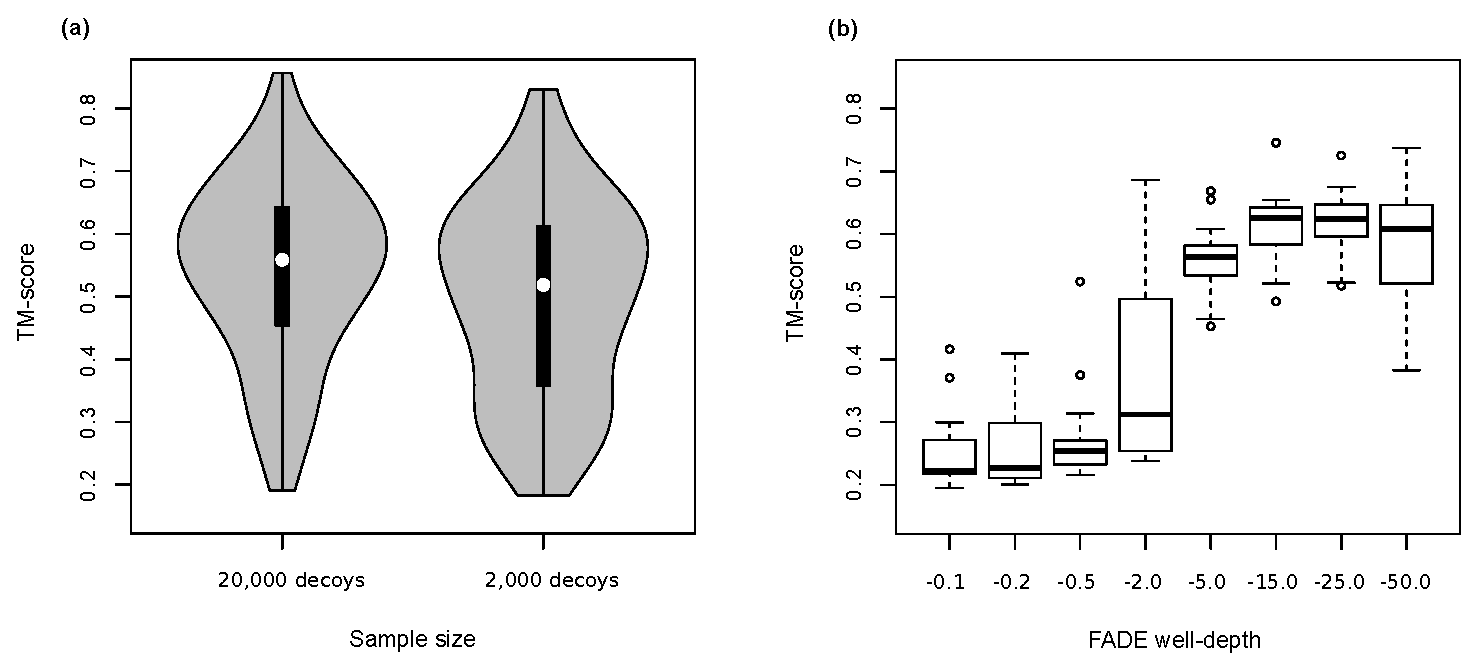
\includegraphics[scale=0.35]{figures/rosetta.eps}}
\caption{Predicted model quality in TM-score for adjustments of two different Rosetta parameters. Reducing the sample size in (a) from 20,000 to 2,000 decoy structures results in reduced native-likeliness of predicted models. However, it also provides a 10-fold speed-up. In (b) we adjust the depth parameter of the FADE function, used to score predicted contacts during folding. A larger absolute value increases the weight of such constraints and results in improved predictions.}\label{fig:ros}
\end{figure}
We selected the FADE function to incorporate predicted residue contacts into Rosetta's native energy function. We then adjusted the parameter $w$ (well-depth) of FADE (Equation \ref{eq:fade}) on a subset of 14 Proteins (Supplementary Table T3) of the PSICOV dataset. The resulting TM-scores are shown in Figure \ref{fig:ros} (b). The energy term from spatial constraints diminishes with well-depth values of -0.5 and above. This leads to a significant decrease in model quality. Lower values of -5.0 and below put a larger absolute weight on the constraints resulting in higher model qualities. We assume this is due to the small number of decoys we are generating in this experiment. We selected a value of -15.0 to achieve high model quality without outweighing Rosetta's native energy function completely.\\\indent
With any number of contacts used during structure prediction, the resulting model quality is on average higher than it would be without contact information. Figure \ref{fig:main} (a) shows average TM-scores for varying amounts of constraints. For each protein the number of top ranked contacts was selected relative to its sequence length. A value of 1.0 on the $x$-axis in Figure \ref{fig:main} (a) represents one contact per residue on average. The same Rosetta protocol as in PconsFold (green circles) was also applied to contacts from PSICOV (black squares) and plmDCA (blue triangles). Comparing $x=0.0$ to any other $x$ shows that predicted contacts generally improve model quality, regardless of method or amount of contacts. \\\indent
Improvements in contact prediction methods also increase the quality of predicted structures. With a maximal average TM-score of 0.55 PconsFold, i.e. using PconsC contacts, provides a 10\% improvement over using PSICOV or plmDCA contacts. This observation is consistent with a direct comparison of contact prediction methods as in \citeauthor{skwark_pconsc:_2013} \citeyear{skwark_pconsc:_2013}. However, the performance difference between PSICOV and plmDCA diminishes when their contacts are used in structure prediction. \\\indent
There is an optimal number of contacts, specific to the contact prediction method. In Figure \ref{fig:main} (a) the maximal average TM-score is reached at $x=1.0$ for PconsFold. For Rosetta/PSICOV and Rosetta/plmDCA a smaller number of one contact every other residue on average is optimal. This can also be explained by the quality of predicted contacts. A larger number of top ranked contacts is predicted with a higher quality in PconsC compared to plmDCA or PSICOV \cite[]{skwark_pconsc:_2013}. Using more of these contacts during structure prediction leads to improved models. \\\indent
This relation between contact and model quality can also be observed in Figure \ref{fig:main} (b). For each protein in the dataset the PPV of its contact map is plotted against the TM-score of the resulting model. The overall Pearson correlation between PPV and TM-score in this dataset is 0.59. Proteins with contact maps of lower quality tend to be modeled less accurate. \\\indent
Proteins belonging to the {\it mainly alpha} CATH fold class seem to be easier to fold than proteins from the {\it alpha \& beta} fold class and proteins from the {\it mainly beta} fold class seem to be hardest to fold. The fold classes are indicated by the color scheme in Figure \ref{fig:main} (b). Predicted contact maps in mainly $\alpha$-helical proteins (blue) have similar or lower PPV values than those of $\beta$-sheet containing proteins (green and yellow), but the resulting models are more accurate in terms of TM-score.
\begin{figure}[!tpb]%figure1
\centerline{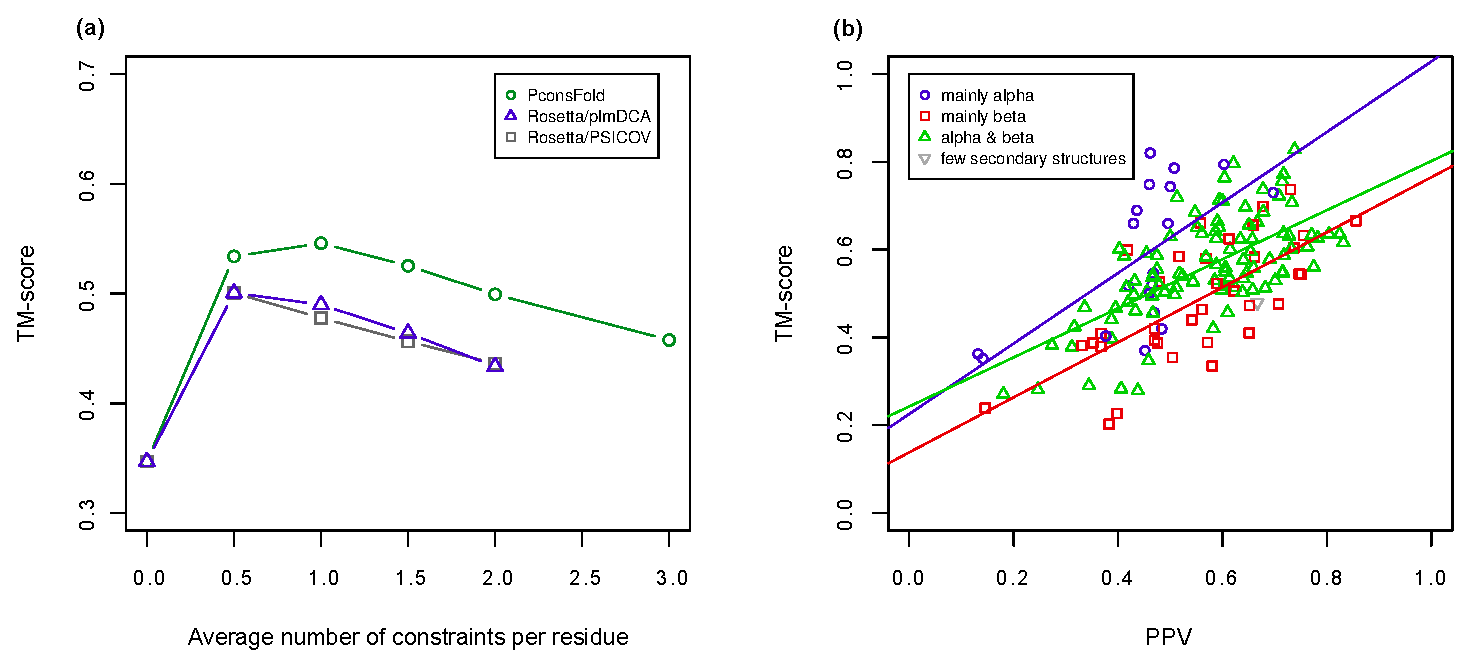
\includegraphics[scale=0.35]{figures/tmscores.eps}}
\caption{In (a) the number of contacts used in structure prediction is plotted against average TM-score for three different methods: PconsFold (green circles), Rosetta/plmDCA (blue triangles), and Rosetta/PSICOV (black squares). There is an optimal number of contacts that depends on the contact prediction method. It also shows that increased contact prediction quality improves native-likeliness of predicted models. In (b) TM-scores are compared to the PPV of underlying contact maps for PconsFold (using PconsC). Mainly alpha helical proteins (blue) are easier to fold than alpha/beta or mainly beta sheet containing proteins.}\label{fig:main}
\end{figure}

\subsection{Model quality assessment}
Table \ref{tab:qa} summarizes the evaluation of different MQAPs on the predictions for the PSICOV dataset. It shows average TM-scores for the top-ranked model after re-ranking all models with each MQAP. In all cases the cumulative score for the full protein was used. Due to technical reasons, Rosetta's internal scoring function was not applicable to the models generated by EVfold. For PconsFold and Rosetta/plmDCA the internal scoring was able to pick the best model on average. In case of EVfold, Pcons selected the best models on average. Pcons performed slightly worse than the internal scoring function of Rosetta on the models from PconsFold and Rosetta/plmDCA. ProQ2 did not perform well on EVfold models. This might be due to non-optimal side-chain placement as an artifact from CNS {\bf(??? can we say that?)}. ProQ2 performed slightly worse than Pcons on models from PconsFold and Rosetta/plmDCA. We also tested a combination of both, as in \citeauthor{wallner_pcons.net:_2007} \citeyear{wallner_pcons.net:_2007}. However, the results are omitted since they were not significantly different from those of Pcons alone. DOPE scoring of EVfold models worked almost as good as Pcons, but we observe a strong decline in average model quality for PconsFold and Rosetta/plmDCA. \\\indent
We assume Rosetta scoring worked that well, because predicted contacts are part of the energy function. Models that satisfy predicted contacts most optimally are assigned low energies and thus ranked on top. Figure \ref{fig:qa} shows a typical example of the difference in satisfied constraints between a top- and bottom-ranked model. Constraints shorter than 8 \AA\ (green lines) are assumed to be correctly formed in the model. Contacts above that distance are not formed (red lines). Apart from overall quality differences, the top-ranked structure clearly contains more correctly modeled residue contacts than the bottom-ranked structure.\\\indent

\begin{table}[!t]
\processtable{Average TM-scores for top-ranked models selected by different MQAPs. \label{tab:qa}}
{\begin{tabular}{llll}\toprule
Method & EVfold & PconsFold & Rosetta/plmDCA \\ \midrule
Rosetta & -- & 0.55 & 0.5 \\
Pcons & 0.47 & 0.53 & 0.47 \\
ProQ2 & 0.36 & 0.51 & 0.46 \\
DOPE & 0.46 & 0.36 & 0.32 \\ \botrule
\end{tabular}}{}
\end{table}

\subsection{Comparison to EVfold}
Figure \ref{fig:vs} shows TM-score pairs for each protein in the PSICOV dataset. The TM-score for PconsFold (a) and Rosetta/plmDCA (b) is plotted along the $x$-axis. TM-scores for EVfold are plotted on the $y$-axis. 
\begin{figure}[!tpb]%figure1
\centerline{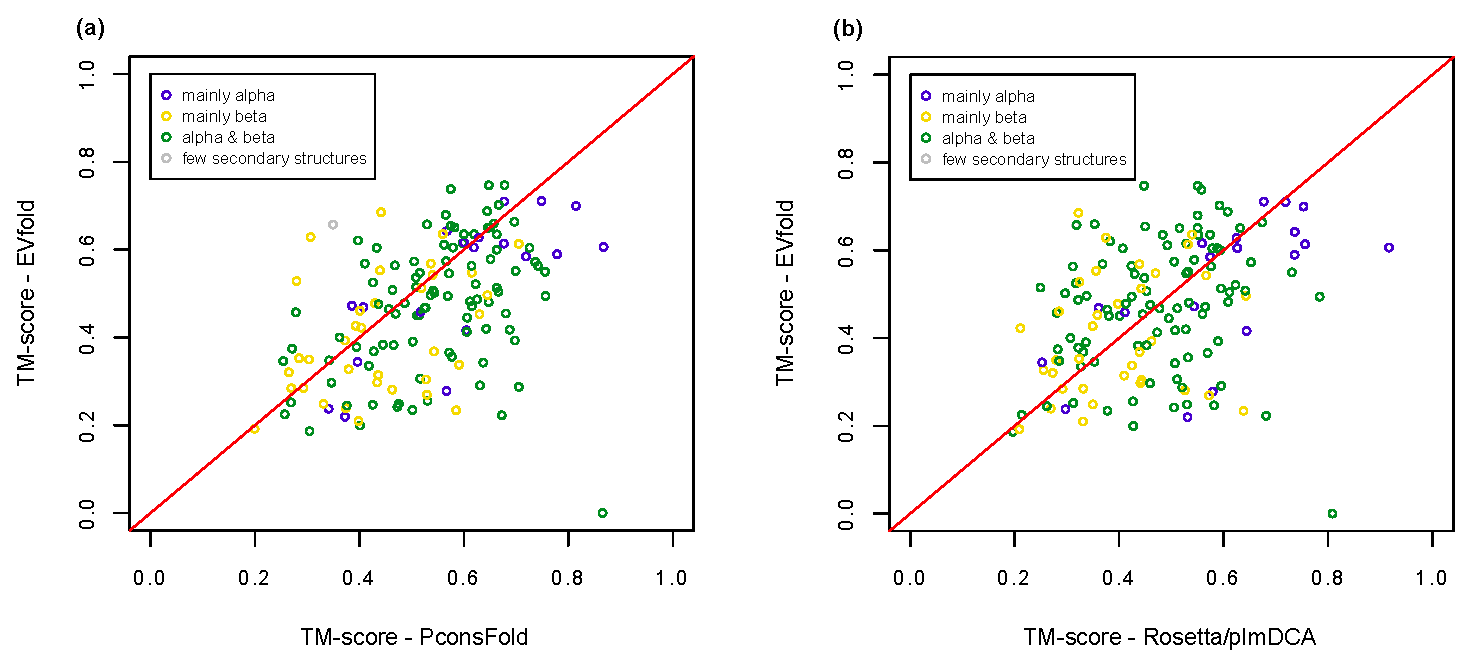
\includegraphics[scale=0.35]{figures/vs.eps}}
\caption{TM-score comparison for all proteins in the PSICOV dataset. The decoys for each method were re-ranked using Pcons. In (a) PconsFold is compared to EVfold. Most of the alpha helical proteins (blue) have higher TM-scores for PconsFold. Most of the proteins where EVfold performs better contain beta sheets (green) or are mainly beta (yellow). Rosetts/plmDCA and EVfold are compared in (b). Both methods perform very similar on average, but there is high divergence when looking at each protein.}\label{fig:vs}
\end{figure}

\begin{table*}[!t]
\processtable{TM-scores for top ranked models comparing EVfold as it was published, current EVfold server (accessed Feb. 2014), EVfold results reranked with Pcons, PconsFold 2,000 decoys, PconsFold 2,000 decoys re-ranked with Pcons, and PconsFold 20,000 decoys. {\bf Add columns for pcons qa and 20k pconsfold}\label{tab:evfold}}
{\begin{tabular}{lllllll}\toprule
Protein & EVfold (paper) & EVfold (web) & EVfold (Pcons ranking) & PconsFold & PconsFold (Pcons ranking) & PconsFold (20k decoys)\\\midrule
%~ & (paper) & (web) & (re-ranked) & (2k decoys) & (2k dec., re-ranked) & (20k decoys) \\ \midrule
BPT1\_BOVIN & 0.49 & 0.25 & 0.5 & 0.44 & ~& ~ \\
CADH1\_HUMAN & 0.55 & 0.54 & 0.6 & 0.59 & ~& ~ \\
CD209\_HUMAN & 0.39 & 0.64 & 0.62 & 0.48 & ~& ~ \\
CHEY\_ECOLI & 0.65 & 0.66 & 0.74 & 0.82 & ~& ~ \\
ELAV4\_HUMAN & 0.57 & 0.61 & 0.57 & 0.74 & ~& ~ \\
O45418\_CAEEL & 0.48 & 0.62 & 0.62 & 0.62 & ~& ~ \\
OMPR\_ECOLI & 0.35 & 0.44 & 0.47 & 0.59 & ~& ~ \\
OPSD\_BOVIN & 0.5 & 0.55 & 0.58 & 0.47 & ~& ~ \\
PCB1\_HUMAN & 0.25 & 0.43 & 0.42 & 0.59 & ~& ~ \\
RASH\_HUMAN & 0.7 & 0.62 & 0.6 & 0.56 & ~& ~ \\
RNH\_ECOLI & 0.54 & 0.66 & 0.66 & 0.64 & ~& ~ \\
SPTB2\_HUMAN & 0.37 & 0.51 & 0.5 & 0.7 & ~& ~ \\
THIO\_ALIAC & 0.55 & 0.56 & 0.61 & 0.79 & ~& ~ \\
TRY2\_RAT & 0.53 * & 0.78 & 0.78 & 0.5 & ~& ~ \\
YES\_HUMAN & 0.35 & 0.31 & 0.37 & 0.63 & ~& ~ \\ \midrule
Mean & 0.48 & 0.55 & 0.57 & 0.61 & ~& ~ \\ \botrule
\end{tabular}}{* This value needed to be corrected to the TM-score of the top-ranked model. In the original publication it showed the value for the best possible model.}
\end{table*}

\section{Conclusion}


\section*{Acknowledgement}
%Text Text Text Text Text Text Text Text. \citealp{Boffelli03} might want to know about text text text text

\paragraph{Funding\textcolon} %Text Text Text Text Text Text Text Text.

\bibliographystyle{natbib}
%\bibliographystyle{achemnat}
%\bibliographystyle{plainnat}
%\bibliographystyle{abbrv}
%\bibliographystyle{bioinformatics}
%
%\bibliographystyle{plain}
%
\bibliography{pcons_fold}


%\begin{thebibliography}{}
%\bibitem[Bofelli {\it et~al}., 2000]{Boffelli03} Bofelli,F., Name2, Name3 (2003) Article title, {\it Journal Name}, {\bf 199}, 133-154.

%\bibitem[Bag {\it et~al}., 2001]{Bag01} Bag,M., Name2, Name3 (2001) Article title, {\it Journal Name}, {\bf 99}, 33-54.

%\bibitem[Yoo \textit{et~al}., 2003]{Yoo03}
%Yoo,M.S. \textit{et~al}. (2003) Oxidative stress regulated genes
%in nigral dopaminergic neurnol cell: correlation with the known
%pathology in Parkinson's disease. \textit{Brain Res. Mol. Brain
%Res.}, \textbf{110}(Suppl. 1), 76--84.

%\bibitem[Lehmann, 1986]{Leh86}
%Lehmann,E.L. (1986) Chapter title. \textit{Book Title}. Vol.~1, 2nd edn. Springer-Verlag, New York.

%\bibitem[Crenshaw and Jones, 2003]{Cre03}
%Crenshaw, B.,III, and Jones, W.B.,Jr (2003) The future of clinical
%cancer management: one tumor, one chip. \textit{Bioinformatics},
%doi:10.1093/bioinformatics/btn000.

%\bibitem[Auhtor \textit{et~al}. (2000)]{Aut00}
%Auhtor,A.B. \textit{et~al}. (2000) Chapter title. In Smith, A.C.
%(ed.), \textit{Book Title}, 2nd edn. Publisher, Location, Vol. 1, pp.
%???--???.

%\bibitem[Bardet, 1920]{Bar20}
%Bardet, G. (1920) Sur un syndrome d'obesite infantile avec
%polydactylie et retinite pigmentaire (contribution a l'etude des
%formes cliniques de l'obesite hypophysaire). PhD Thesis, name of
%institution, Paris, France.

%\end{thebibliography}
\end{document}

